\documentclass[a4paper]{article}
\usepackage[english]{babel}
\usepackage{multicol}
\usepackage{amsmath}
\usepackage{amsfonts}
\usepackage{amssymb}
\usepackage{graphicx}
\usepackage[font=scriptsize]{caption}
\usepackage{parskip}
\usepackage[a4paper, margin= 1in ,total={6in, 8in}]{geometry}
\usepackage{titling}
\usepackage{subcaption}
\usepackage{float}
\usepackage{placeins}

\parskip = 6pt plus 2pt minus 2pt
\setlength{\droptitle}{-2cm}

\title{HW1- Computer Simulation II}
\author{Schewtschik, Guilherme  (3748052)}
\date{\today}

\begin{document}
\maketitle

\section{}
In the first attempt, the Metropolis algorithm was used, but it became clear that for a lattice larger than $8 \times 8$ the run time around the critical temperature became too large, so instead the Wolff algorithm was chosen.
With this we arrive at the following graph:

\begin{figure}[H]
    \centering
    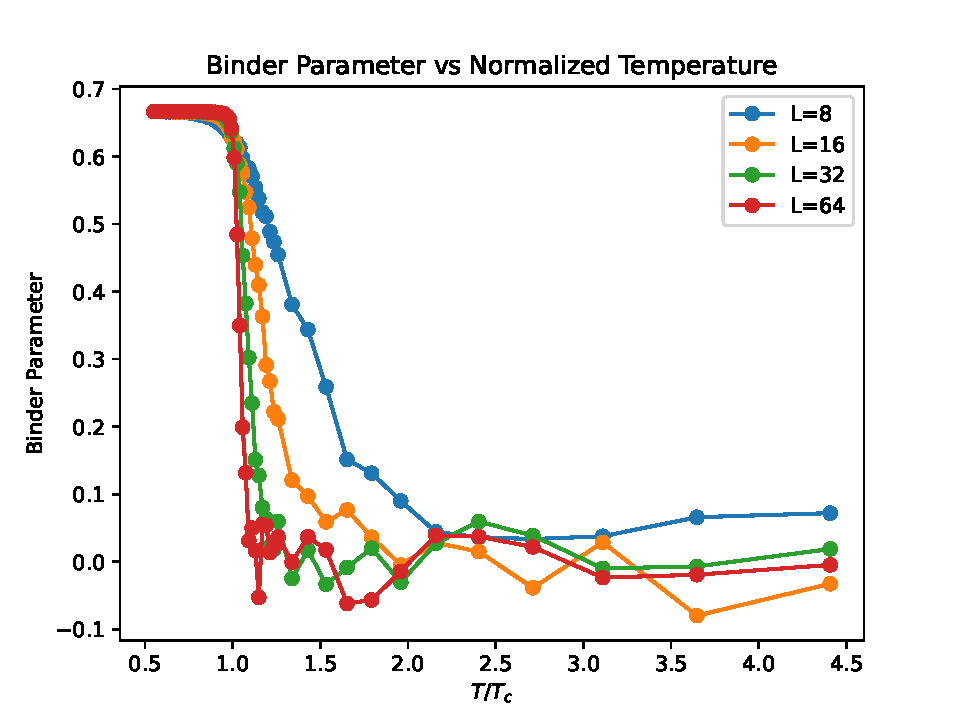
\includegraphics[width=0.65\linewidth]{plots/U_T.pdf}
    \caption{BinderXT}
    \label{fig:U}
\end{figure}

We can see that the value for $U$ stays the similar for all $L$ until reaching the critical temperature where they diverge.

Plotting the difference between the data points we get:

\begin{figure}[H]
    \centering
    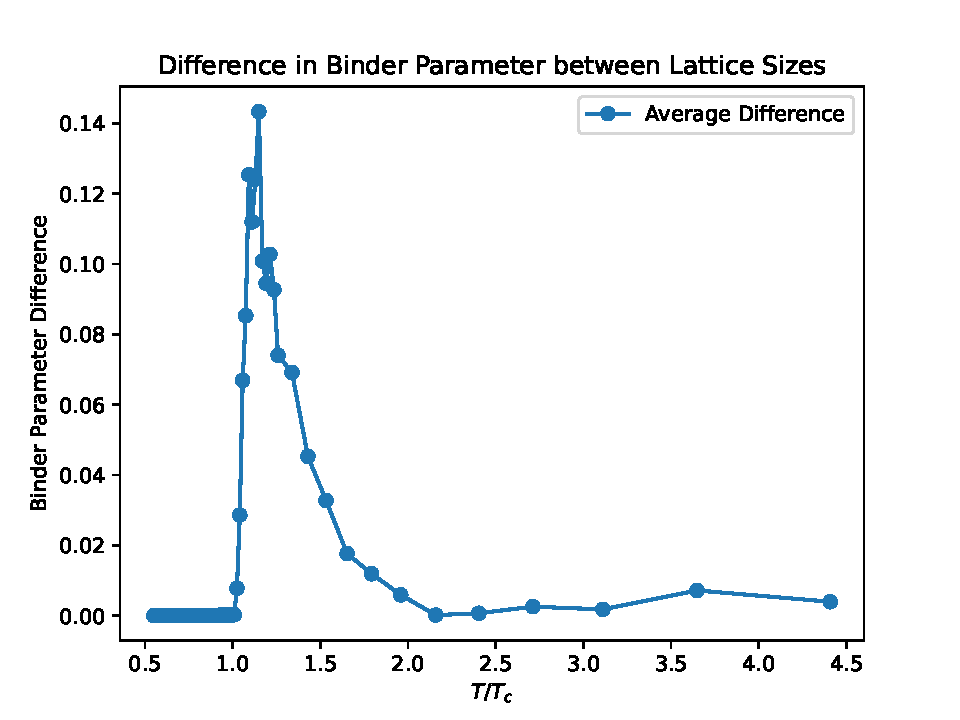
\includegraphics[width=0.65\linewidth]{plots/diff_U.pdf}
    \caption{Caption}
    \label{fig:placeholder}
\end{figure}

We can also see to a lower extent a convergence at higher temperatures. 

The estimated value for $U$ at $T/T_c$ is:
\begin{verbatim}
    Estimated U at T_c: L=8: 0.630, L=16: 0.628, L=32: 0.637, L=64: 0.641
    Mean U at T_c: 0.634
\end{verbatim}

\FloatBarrier

\section{}
Calculating the value of $\chi$ we can clearly see the peaks around the critical temperature:

\begin{figure}[H]
    \centering
    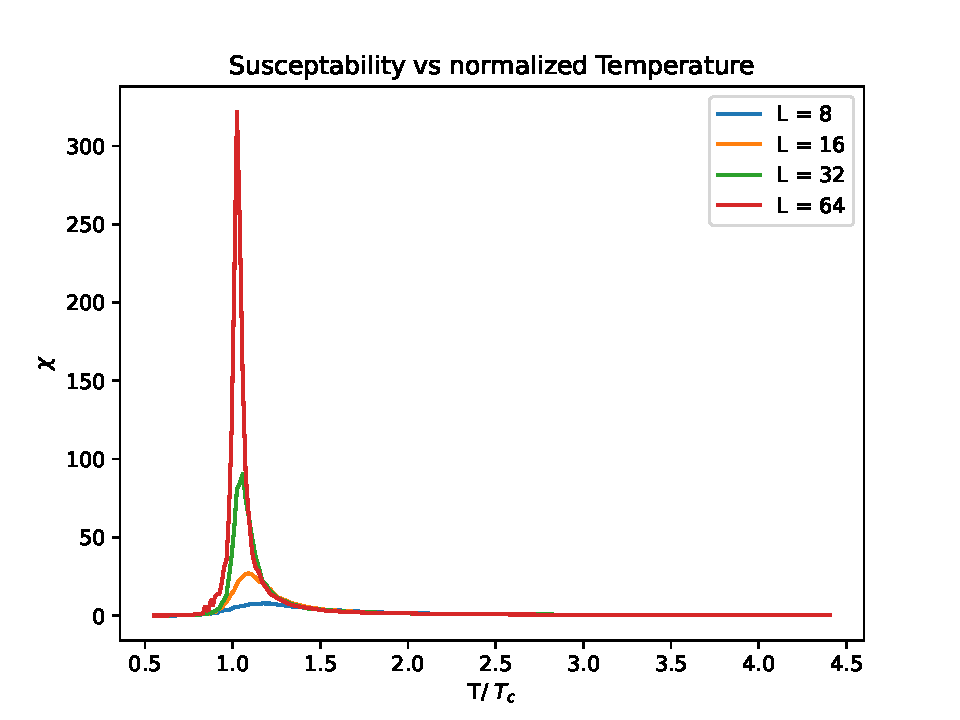
\includegraphics[width=0.65\linewidth]{plots/chi.pdf}
    \caption{$\chi$ values}
    \label{fig:placeholder}
\end{figure}

Taking the maximum of $\chi$ and plotting it against the lattice size $L$, we can see the relation between them appears to be exponential:

\begin{figure}[H]
    \centering
    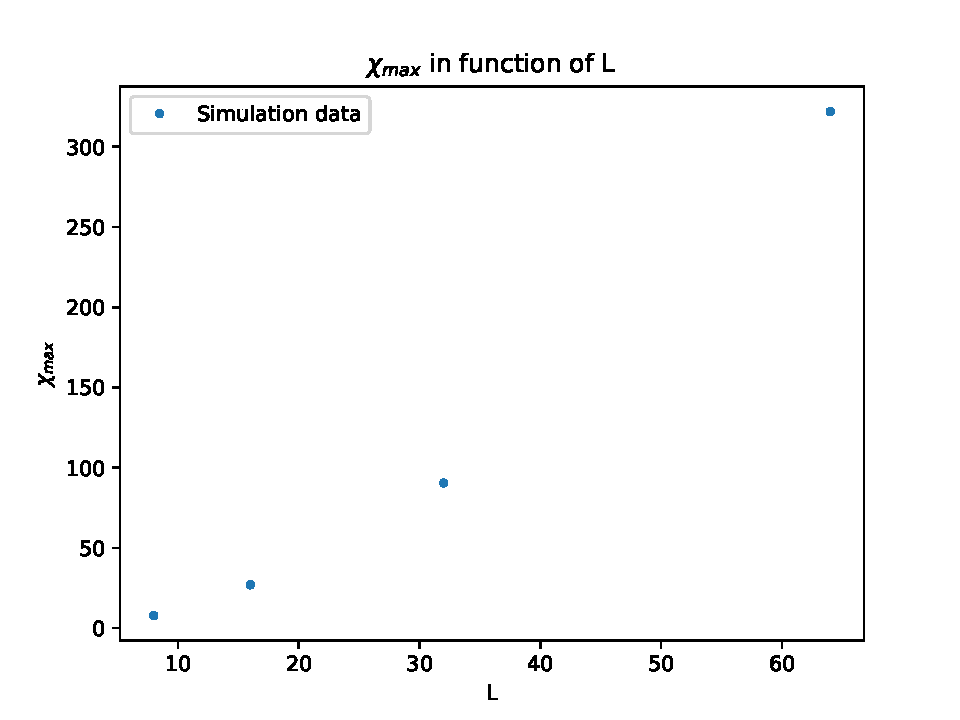
\includegraphics[width=0.65\linewidth]{plots/chi_max.pdf}
    \caption{$\chi$ in function of $L$} 
    \label{fig:placeholder}
\end{figure}
\newpage
For us to test the finite-size scaling Ansatz, we first need to make some adjustments, instead of using the given formula we shall work in log space:

\begin{equation}
    ln(\chi) = \frac{\gamma}{\nu}ln(L) + c
\end{equation}

Where $c$ is a proportionality constant. Using this equation and 
fitting a line we can find the values for $\gamma/ \nu$ and $c$.

\begin{align}
    \frac{\gamma}{\nu} = 1.783169... \quad c = - 1.65374
\end{align}
    
\begin{figure}[H]
    \centering
    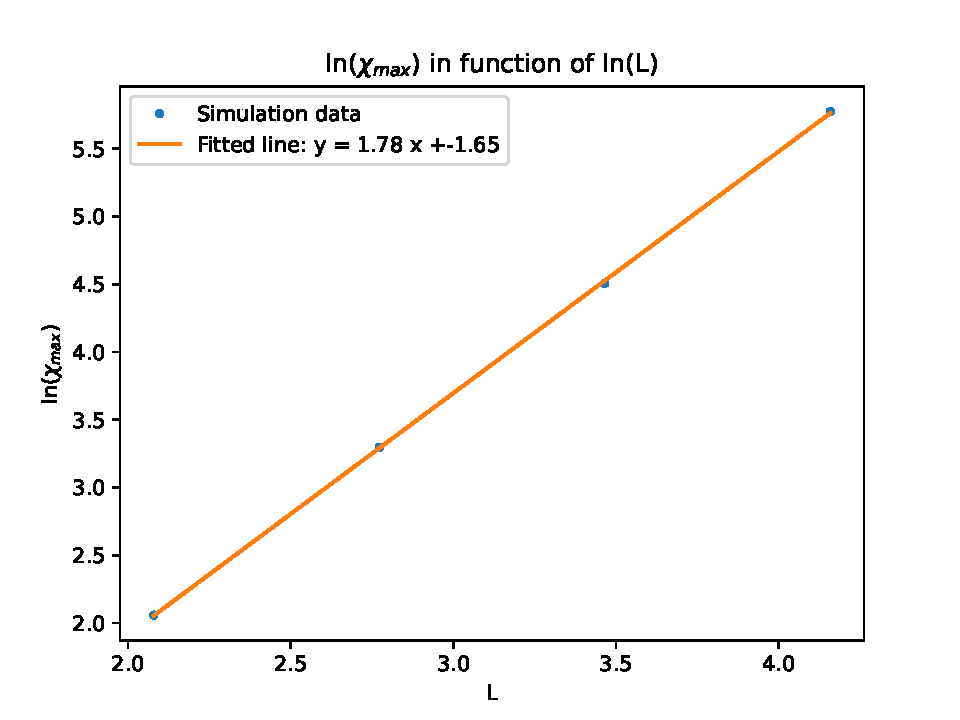
\includegraphics[width=0.7\linewidth]{plots/ln_chi.pdf}
    \caption{Fitted $\chi_{max}$}
    \label{fig:placeholder}
\end{figure}

\FloatBarrier

\end{document}
